\chapter{評価}\label{ch:evaluation}

\section{評価手法}\label{sec:methodology}

例えばここでは評価に用いたハードウェアやソフトウェアについて説明をする。
表を用いると効果的なことが多いので積極的に活用する。

\begin{table}[ht]
  \caption{数字が色々書いてある表}{
  \centering
  \resizebox{0.95\textwidth}{!}{
    \begin{tabular}{c  c c c  c c c}
      \toprule
比較 & \multicolumn{3}{c}{何かの結果} & \multicolumn{3}{c}{何かとの比較} \\
対象  & 面積($mm^2$) & 遅延($ns$)  & 電力($m W$)    & 面積(\%)  & 遅延(\%) & 電力(\%) \\
      \midrule
ベースライン & 347,329.19 & 1.62 & 15.84 & --- & --- & --- \\
      \midrule
提案手法1 & 412,263.87 & 1.65 & 16.17 & 18.69 & 1.85 & 2.12 \\
      \midrule
提案手法2 & 370,972.35 & 2.42 & 17.95 & 6.80 & 49.38 & 11.00 \\
      \midrule
提案手法3 & 356,694.82 & 1.98 & 16.00 & 2.69 & 22.22 & 1.06 \\
      \bottomrule
    \end{tabular}\label{tab:example}
  }
}
\end{table}

\cref{tab:example}には色々な数字を示してある。
なお表には縦線を入れない方が見た目はすっきりしていて綺麗である(リンタの下記メッセージを見たことがある人もいるのではなかろうか:``Vertical rules in tables are ugly.'')。

\section{評価結果}\label{sec:results}

評価結果を定量的に示し、考察などを行なう。
グラフを用いること効果的なことが多いので積極的に活用する。

\begin{figure}[ht]
  \centering
  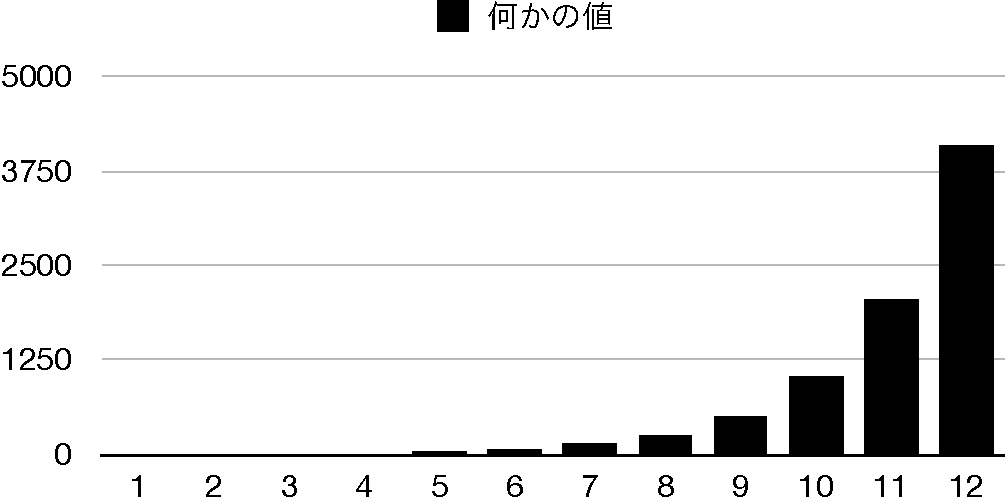
\includegraphics[width=0.9\textwidth]{examples/graphs/example}
  \caption{何かの値}\label{fig:example}
\end{figure}

\cref{fig:example}を見ると、何かの値が指数的に増加していることが分かる。
評価結果の詳細なデータを\cref{ch:appendix2}に示す。